\documentclass[a4paper,11pt]{article}

\usepackage[latin1]{inputenc}
\usepackage[T1]{fontenc}
\usepackage{bbm} %math chars
\usepackage{amsmath}
\usepackage{indentfirst}
\usepackage{fullpage} %minimizes the default margins
\usepackage{url}
\usepackage{graphicx}
\usepackage[center,footnotesize]{caption} %options des legendes des graphes
\usepackage[section]{placeins} %place les figures d'une section avant le debut de la suivante
\usepackage{subfig} %a) b) c)
\usepackage{fancyvrb}

\title{Exercises - Week 10}
\date{}
\author{Genomics and bioinformatics}

\begin{document}
\maketitle

\indent In this series, you will be handling real biological data to replicate figures in a published paper. You can find the pdf file of the paper on moodle, or you can access it online through the following link:

\url{http://www.nature.com/nature/journal/v469/n7330/full/nature09652.html}

\section{Background}
\indent The central dogma of molecular biology states that the flow of information within a biological system goes from DNA to RNA to protein. The first step in gene expression, transcription, is the process where the genomic DNA sequence is converted to a complementary RNA sequence through a complex machinery involving RNA polymerases. It is one of the most fundamental processes linking genotype to phenotype in all life forms. In humans, however, 80\% of the genome is transcribed but only 1\% codes for proteins. For that reason, in order to understand how biological systems work, it is important to understand the first step of gene expression.

\indent Traditionally, it was thought that transcription starts at a gene's transcription start site, then proceeds without stopping until a full pre-mRNA is produced when it is subsequently processed into the mature form. Now it is becoming clear that these processes  occur simultaneously and that many transcripts are produced and degraded quickly, thus never reaching maturity.

\indent The existing tools that measure gene expression, namely microarrays and RNA-sequencing, target mature forms of RNA and do not detect the immature RNA transcripts. In the paper by Churchman and Weissman, a new approach was proposed to  precisely quantify transcripts as they are being produced. In native elongating transcript sequencing (NET-seq) only the RNA that is bound to RNA polymerase (RNAP) is sequenced, enabling the study of rapidly-degraded transcripts, the identification of RNAP pause sites and the factors regulating transcription events. They apply this technique and standard RNA-seq on wild-type and mutant strains of \textit{Saccharomyces cerevisiae} (budding yeast) to understand transcription elongation dynamics.

\section{Getting the data}
\indent In most genomics papers, the actual data is stored in databases with unique accession codes. For this paper, the data can be found in different NCBI databases:
\begin{itemize}
\item BioProject (\url{http://www.ncbi.nlm.nih.gov/bioproject})
\item BioSample (\url{http://www.ncbi.nlm.nih.gov/biosample/})
\item SRA (\url{http://www.ncbi.nlm.nih.gov/sra})
\item Gene Expression Omnibus (\url{http://www.ncbi.nlm.nih.gov/geo/})
\end{itemize}

 Find the accession codes for this paper's dataset and then go to the appropriate database.

\begin{enumerate}
\item From which database would you download the raw sequencing files?
\item From which database would you get general information about a specific sample?
\item What is the difference between the datasets in SRA and those in GEO?
\end{enumerate}

\section{Viewing the data in UCSC}
To save time, we have included the appropriate datafiles from GEO in the Moodle. We have only taken the expression data of chromosome VII to reduce file size. Go to the UCSC genome browser and click on "Genomes". You will need to select sacCer2 assembly of \textit{S. cerevisiae}. The datafiles are in a format called "wiggle", which is supported by UCSC genome browser. This is the head of one of the files:
\newline
\newline
\noindent\texttt{track type=wiggle\_0 name=WT\_NC\_plus\newline
variableStep chrom=chrVII\newline
1930 0.481987825759\newline
2772 0.963975651517\newline
2786 0.963975651517\newline
2790 1.44596347728\newline
2800 0.481987825759\newline}

The first two lines are used by UCSC to know the type of data, the name of the track, and on which chromosomes the data is supposed to be. Each line after that contains two values: the first indicates the location on the chromosome and the second indicates the number of reads per 10\textsuperscript{7} total reads that have mapped to that location.

You can add those files as custom tracks by clicking on "manage custom tracks" and uploading the ".wig" file.
\begin{enumerate}
\item In figure 1b in the paper, the authors show a proof of principle of their NET-seq protocol by comparing it to RNA-seq. Upload the appropriate tracks to the genome browser and zoom to the RPL30 gene (YGL030W). Do you get the same result?
\item The authors talk about CUTs in the paper. What are they?
\item Visualize the CUTs in the cluster of genes in figure 3a (make sure you upload the appropriate tracks). What do you notice when you compare \textit{RCO1$\Delta$} to the wild-type?
\item For the next exercise, you will need to extract gene annotation information (like strand and transcription start) for all the genes on chromosome VII. This is easy to do in UCSC. Go to \textit{Tools}>\textit{Table Browser}. Under \textit{Group}, select \textit{Genes and Gene Prediction Tracks}, then select \textit{SGD Genes} in the track drop down list. Define the position as "chrVII" and then click on get output. Download the resulting table, for this will be useful for the next exercise.
\end{enumerate}

\section{Reproducing figures from the paper}
\begin{enumerate}
\item Try to reproduce figure 1b using an appropriate programming language (we advise R). You will need to load the appropriate ".wig" files and to extract the region corresponding to the RPL30 gene. You will also need to use the table downloaded from UCSC, which contains information about the genes on chromosome VII. Not that in order to use the UCSC file in R, you will need to manually edit the header and remove the "\#" at the beginning so that R does not ignore it.
\item Explain the significance of figure 3b and try to reproduce it. Check the methods section for how the calculations were made. However, we will perform simpler calculations for each gene:
The diagrams below define the way you should perfom the calculations for each gene. 

Remember that genes can be on either strand of the genome, and that what is "sense" for one gene is "antisense" for the other. You might not be able to complete this during the 2 hour session, so try to do it at home. Also note that the data that, unlike the paper, we are working on chromosome VII alone.
\end{enumerate}
\begin{center}
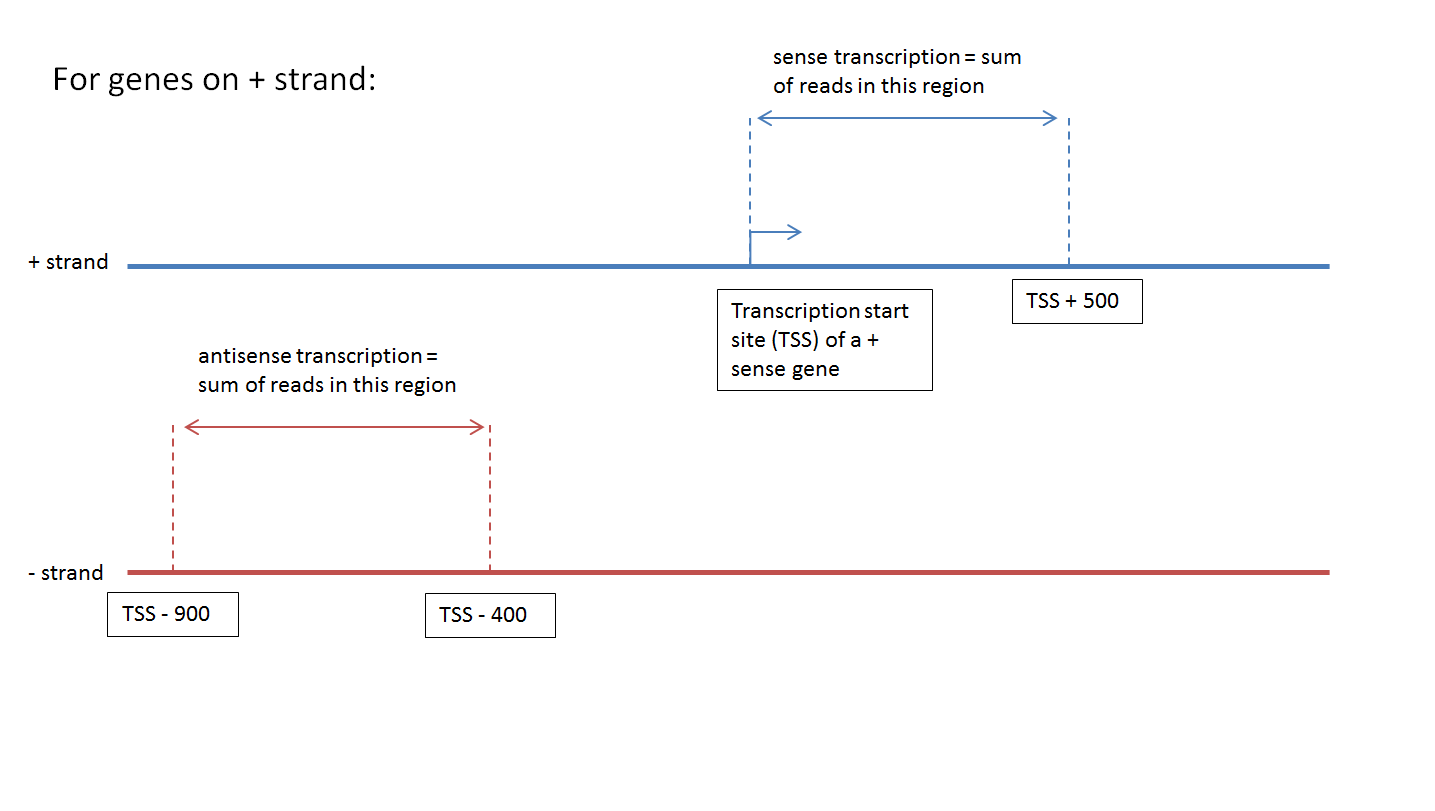
\includegraphics[width=0.9\textwidth]{positive_gene.png}\\
\vspace{0.1cm}
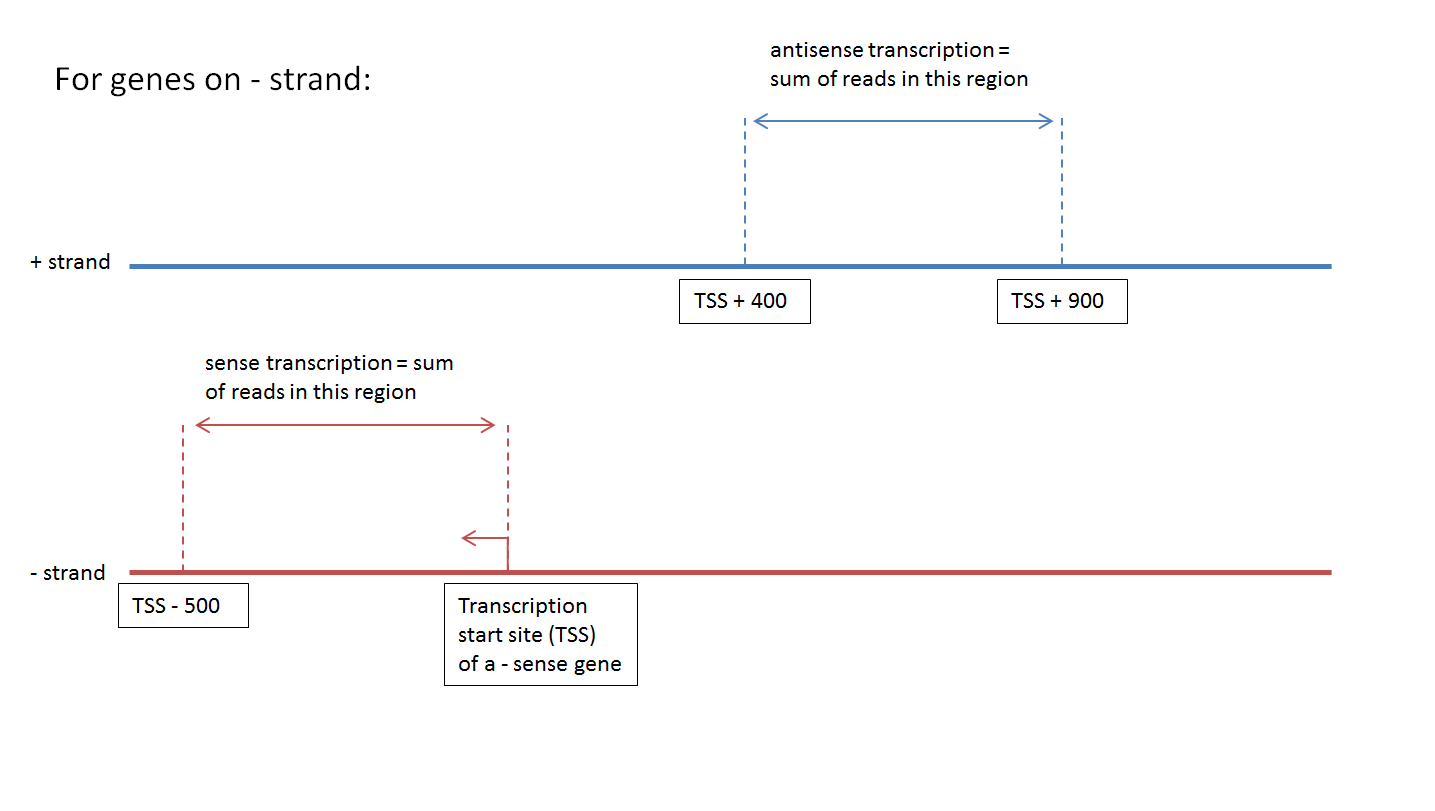
\includegraphics[width=0.9\textwidth]{negative_gene.png}\\
\end{center}

\end{document}











